% board-warping/key.tex — generated by board-warping/tools/board_warping.py; do not edit.
% The colour key of the panels: 12 bands of 0.5 mm from -3 to 3 mm; its width is 0.62 \linewidth.
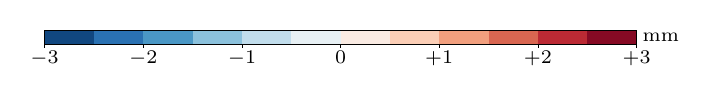
\begin{tikzpicture}[baseline=(current bounding box.north)]
\fill[fill={rgb,255:red,17;green,71;blue,128}] (0*\dimexpr0.62\linewidth/12\relax,0) rectangle (1*\dimexpr0.62\linewidth/12\relax+0.05pt,5pt);
\fill[fill={rgb,255:red,42;green,113;blue,178}] (1*\dimexpr0.62\linewidth/12\relax,0) rectangle (2*\dimexpr0.62\linewidth/12\relax+0.05pt,5pt);
\fill[fill={rgb,255:red,74;green,151;blue,197}] (2*\dimexpr0.62\linewidth/12\relax,0) rectangle (3*\dimexpr0.62\linewidth/12\relax+0.05pt,5pt);
\fill[fill={rgb,255:red,139;green,193;blue,220}] (3*\dimexpr0.62\linewidth/12\relax,0) rectangle (4*\dimexpr0.62\linewidth/12\relax+0.05pt,5pt);
\fill[fill={rgb,255:red,193;green,221;blue,236}] (4*\dimexpr0.62\linewidth/12\relax,0) rectangle (5*\dimexpr0.62\linewidth/12\relax+0.05pt,5pt);
\fill[fill={rgb,255:red,231;green,240;blue,244}] (5*\dimexpr0.62\linewidth/12\relax,0) rectangle (6*\dimexpr0.62\linewidth/12\relax+0.05pt,5pt);
\fill[fill={rgb,255:red,250;green,235;blue,227}] (6*\dimexpr0.62\linewidth/12\relax,0) rectangle (7*\dimexpr0.62\linewidth/12\relax+0.05pt,5pt);
\fill[fill={rgb,255:red,251;green,206;blue,182}] (7*\dimexpr0.62\linewidth/12\relax,0) rectangle (8*\dimexpr0.62\linewidth/12\relax+0.05pt,5pt);
\fill[fill={rgb,255:red,241;green,159;blue,126}] (8*\dimexpr0.62\linewidth/12\relax,0) rectangle (9*\dimexpr0.62\linewidth/12\relax+0.05pt,5pt);
\fill[fill={rgb,255:red,216;green,102;blue,81}] (9*\dimexpr0.62\linewidth/12\relax,0) rectangle (10*\dimexpr0.62\linewidth/12\relax+0.05pt,5pt);
\fill[fill={rgb,255:red,187;green,42;blue,52}] (10*\dimexpr0.62\linewidth/12\relax,0) rectangle (11*\dimexpr0.62\linewidth/12\relax+0.05pt,5pt);
\fill[fill={rgb,255:red,134;green,10;blue,36}] (11*\dimexpr0.62\linewidth/12\relax,0) rectangle (12*\dimexpr0.62\linewidth/12\relax+0.05pt,5pt);
\draw[line width=0.2pt] (0,0) rectangle (12*\dimexpr0.62\linewidth/12\relax,5pt);
\draw[line width=0.2pt] (0*\dimexpr0.62\linewidth/12\relax,0) -- ++(0,-1.5pt) node[below, inner sep=1pt, font=\scriptsize] {${-}3$};
\draw[line width=0.2pt] (2*\dimexpr0.62\linewidth/12\relax,0) -- ++(0,-1.5pt) node[below, inner sep=1pt, font=\scriptsize] {${-}2$};
\draw[line width=0.2pt] (4*\dimexpr0.62\linewidth/12\relax,0) -- ++(0,-1.5pt) node[below, inner sep=1pt, font=\scriptsize] {${-}1$};
\draw[line width=0.2pt] (6*\dimexpr0.62\linewidth/12\relax,0) -- ++(0,-1.5pt) node[below, inner sep=1pt, font=\scriptsize] {$0$};
\draw[line width=0.2pt] (8*\dimexpr0.62\linewidth/12\relax,0) -- ++(0,-1.5pt) node[below, inner sep=1pt, font=\scriptsize] {${+}1$};
\draw[line width=0.2pt] (10*\dimexpr0.62\linewidth/12\relax,0) -- ++(0,-1.5pt) node[below, inner sep=1pt, font=\scriptsize] {${+}2$};
\draw[line width=0.2pt] (12*\dimexpr0.62\linewidth/12\relax,0) -- ++(0,-1.5pt) node[below, inner sep=1pt, font=\scriptsize] {${+}3$};
\node[right, inner sep=2pt, font=\scriptsize] at (12*\dimexpr0.62\linewidth/12\relax,2.5pt) {mm};
\end{tikzpicture}%
